We find that developers use \unsafe code for ergonomics, performance, and when they perceive that there is no alternative. Despite attempts to keep \unsafe code minimal and encapsulated, developers feel uncertain about its correctness. These results mirror findings from Holtervennhoff et al~\cite{holtervennhoff23}, and we compare our results with theirs in Sections~\ref{results:rq1} and~\ref{results:rq2}. Foreign function calls were used by most participants, and non-trivial differences between Rust and other languages made these calls difficult to encapsulate. Developers rarely audited their dependencies. Most had used Miri, but few used it to validate their test cases, and its lack of support for foreign function calls deterred some individuals from using it.

\subsection{Demographics} We invited all \ArrayItem{responses.screening.raw} eligible candidates to participate in interviews, and we interviewed \ArrayItem{responses.screening.valid} who responded to our invitation. Of these participants, \ArrayItem{screening.affiliation.industry} had experience in industry, \ArrayItem{screening.affiliation.open.source} in open source development, \ArrayItem{screening.affiliation.academia} in academia, and \ArrayItem{screening.affiliation.rust.team} were members of the Rust team. They had 4.7 years of experience with Rust on average, and the most experienced participant had been using Rust for 10 years. 

\FPeval{\degree}{round(clip(\ArrayItem{demo.education.bachelor's.degree} + \ArrayItem{demo.education.phd}+\ArrayItem{demo.education.master's.degree}),0)}
\FPeval{\graduatedegree}{round(clip(\ArrayItem{demo.education.phd}+\ArrayItem{demo.education.master's.degree},0))}
\FPeval{\belowforty}{round(clip(\ArrayItem{demo.age.18-29}+\ArrayItem{demo.age.30-39} ),0)}

We received \ArrayItem{responses.survey.raw} survey responses, of which \ArrayItem{responses.survey.finished} were complete, \ArrayItem{responses.survey.without.fraud.detection} met our eligibility criteria, and \ArrayItem{responses.survey.valid} passed each of Qualtrics' measures for fraud detection. Hereafter, when we refer ``respondents,'' we include only those that are eligible. The majority were young, educated, identified as male, and had experience in either industry or open-source development. Nearly \degree\% had completed at least a bachelor's degree, and \graduatedegree\% had completed a graduate degree. Most respondents (\belowforty\%) were younger than 40 years old, and \ArrayItemRounded{demo.age.18-29}\% were between the ages of 18 and 29. We followed Spiel et al.'s~\cite{spiel19_gender} guidelines for ethically surveying respondents' gender; 80\% identified as ``Man'', \ArrayItemRounded{demo.gender.non-binary}\% identified as ``Non-binary,'' \ArrayItemRounded{demo.gender.woman}\% identified as ``Woman'' and \ArrayItemRounded{demo.gender.prefer.not.to.disclose}\% did not disclose their gender. On average, survey respondents had more than a decade of experience in software engineering, more than 5 years of experience in both C and \CC{}, and just over 4 years of experience using Rust.

\subsection{Why unsafe?}
\label{results:rq1}
\begin{figure}
\centering
\caption{How frequently participants measured the impact of their changes when using \unsafe to improve performance}
\label{fig:rq2:profiling}
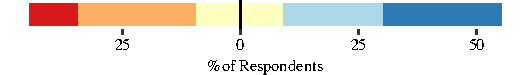
\includegraphics[width=\columnwidth]{figures/compiled/rq2_profiling.pdf}
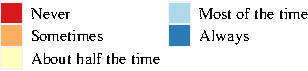
\includegraphics{figures/compiled/legends/legend_frequency_wrapped.pdf}
\end{figure}

Participants used \unsafe code because they perceived that it was more performant or ergonomic than safe alternatives, or that there were no safe alternatives at all.

\subsubsection{Unsafe Performs Better}
Some interview participants and \ArrayItemRounded{rq2.motivation.i.could.use.a.safe.pattern.but.unsafe.is.faster.or.more.space-efficient.}\% of survey respondents indicated that they would use \unsafe code when they perceived that it was faster or more space-efficient than an equivalent safe API. In these situations, participants usually identified a safe alternative, but they felt that it would be too expensive to use; \ilquote{so you could do it, right? But that would be some performance overhead}{12}. 

Most interview participants who attempted to use \unsafe to improve performance had implemented small-scale optimizations in existing applications. These typically involved eliminating runtime checks, which were seen as unnecessary due to local or global invariants. For example, one participant used an \unsafe API to consume a pointer to a string without checking if it contained valid UTF-8 characters. This pointer was provided by a foreign call to Python, which the participant reasoned would only ever provide text in a valid format. Another participant chose to store a heap allocation as a raw pointer in a static mutable variable instead of using one of Rust's safe static encapsulations, since they felt confident that the allocation would be valid for the duration of the program.


However, a few interview participants used \unsafe code to create entire components that were purpose-built to achieve performance.  In each situation, performance was seen as a functional requirement for the application domain: \ilquote{I write a serialization framework...And obviously a goal for it is to be extremely performant}{3}. A participant who took this approach found that it significantly increased the amount of \unsafe code in their application, but they felt that this was a reasonable compromise to achieve greater performance.

The \ArrayItemRounded{rq2.motivation.i.could.use.a.safe.pattern.but.unsafe.is.faster.or.more.space-efficient.}\% of survey respondents who reported using \unsafe code to improve performance did not have a strong tendency toward either large-scale or small-scale use. We found that \ArrayItemRounded{rq2.perf.scale.small-scale.optimizations}\% only pursued ``small-scale-optimizations in existing applications,'' \ArrayItemRounded{rq2.perf.scale.large-scale.components.purpose-built.for.performance.}\% only built new, ``large-scale components,'' and \ArrayItemRounded{rq2.perf.scale.both}\% used \unsafe code for performance in either situation.

\FPeval{\profilingmore}{round(\ArrayItem{rq2.profiling.about.half.the.time} + \ArrayItem{rq2.profiling.always} + \ArrayItem{rq2.profiling.most.of.the.time}, 0)}

Participants did not consistently measure the performance impact of \unsafe code. In some situations, they relied on their intuition to determine which design decisions would be best: \ilquote{I'll totally admit that...I think this is going to be a hot thing, so I'm going to kind of prematurely optimize}{11}. Survey respondents who used \unsafe to increase performance were also inconsistent about measuring its impact. However, \profilingmore\% reported measuring performance at least half the time or more, as shown in Figure~\ref{fig:rq2:profiling}. Similarly, Höltervennhoff et al.~\cite{holtervennhoff23} found that 6 participants would use \unsafe code to improve performance when the change was ``noticeable.'' One of our interview participants performed sophisticated profiling on three versions of a component, each of which had varying amounts of \unsafe. The most \unsafe-heavy version performed the best, but they opted for one with a moderate amount of \unsafe code, balancing concerns for safety and performance. 

\subsubsection{Unsafe is Easier or More Ergonomic}
Participants also chose to use \unsafe code when they felt it would be easier than using a safe API. This was the least common motivation cited by interview participants, and only \ArrayItemRounded{rq2.motivation.i.could.use.a.safe.pattern.but.unsafe.is.easier.to.implement.or.more.ergonomic.}\%  of survey respondents identified with this motivation. Höltervennhoff et al.\cite{holtervennhoff23} indicate that some of their participants would use unsafe code if it ``saved them effort'', but it was unclear if this motivation was typical. Our participants usually stated or implied a choice between using safe or \unsafe design patterns. For example, one participant chose to use only Rust's \unsafe allocator API rather than a mix of \unsafe and safe allocation operations. They found that this approach was easier to reason about, since \ilquote{if there's too much abstraction, you lose the information that you need to make it actually sound}{4}.

The \unsafe function \code{transmute} performs unrestricted type conversion, and it was used by several participants to circumvent safe APIs that they found were difficult to use. One participant used transmutation to simplify the implementation of chess engine, which had three enumerations to represent the position of a chess piece. They found that it was easier to use integer conversion, bitwise operations, and transmutation to convert between enumerations instead of safely matching on their values. Another participant used transmutation when working with a Rust encapsulation of a C font library. This library exposed C heap allocations as Rust object with short lifetimes\textemdash even though these objects would remain valid on the heap for the duration of the program. This participant found it was easier to transmute the Rust objects to have the \code{{\textquotesingle}static} lifetime, which is indefinite, instead of adapting to the restrictions of the encapsulation. 
\begin{pquote}{14}
I just...transmuted that one to {\normalfont \code{{\textquotesingle}static}}...
another use case for {\normalfont \unsafe} is working around a bad API when you know that you can use it correctly.
\end{pquote}

\FPeval{\impossible}{round(\ArrayItem{rq2.impossibility.most.of.the.time} + \ArrayItem{rq2.impossibility.always},0)}

\subsubsection{No Clear Alternative}
In most situations, participants perceived that they had no clear alternative to using \unsafe code. The majority of interview participants and \ArrayItemRounded{rq2.motivation.i.am.not.aware.of.a.safe.alternative.at.any.level.of.ease-of-use.or.performance.}\% of survey respondents identified with this motivation. Höltervennhoff et al.\cite{holtervennhoff23} observed this to a similar extent; 18 out of their 26 participants claimed to use \unsafe code by necessity. Our interview participants often reported being constrained by a combination of Rust's type system and the properties of their applications. For example, in Rust, if a type implements the \unsafe traits \code{Send} and \code{Sync}, then users can freely use and share its values in multithreaded contexts. One participant found that it was necessary to implement \code{Send} and \code{Sync} in a single-threaded application to maintain compatibility with an existing API. The implementation was sound by construction, but \unsafe was still necessary.

Participants who contributed to just-in-time (JIT) compilers and operating systems found it necessary to access memory through raw pointers. This was necessary for one participant to implement an unwinding table: \ilquote{I have to jump to that address and I really can't do anything to verify it...}{12}. In other situations, developers felt that there could be a safe alternative, but they were unaware of how to implement it: \ilquote{there's probably a better way that I just don't know about yet or didn't know about at the time and I haven't thought about it}{18}. However, \impossible\% of survey respondents were certain at least most of the time, if not always, that it would be impossible to implement an equivalent safe pattern.

\subsubsection{Co-occurrence} These motivations were not mutually exclusive. One participant implemented a zero-copy deserialization pattern using \unsafe code, and their experience relates to each of the reasons we identified. Performance was a domain-specific constraint of the internationalization library that they contributing to, which motivated them to use zero-copy deserialization. We reviewed the library's documentation, and it indicated that contributors had considered using an existing crate, but its API was not ergonomic for their use case. The participant decided to implement their own version, and they perceived that \unsafe code was inherently necessary.

\label{response:rq1}
\rsqtwo Participants were most often motivated to use \unsafe code because they felt that there was no safe alternative. In other situations, participants used \unsafe code because it performed better or was more ergonomic. For performance, developers pursued both large-scale abstractions and small-scale optimizations, but they did not consistently measure the impact of their changes. Each of these motivations can influence a design decision simultaneously.

\subsection{Design \& Use of Unsafe APIs}
\label{results:rq2}
\subsubsection{Invariants}
Participants reasoned about the soundness and correctness of their \unsafe code in terms of invariants.  When developing operating systems and embedded applications, certain invariants were provided by hardware specifications. For example, one participant who developed an embedded application would write a \ilquote{magic value}{8} to RAM to indicate which operation had triggered a reboot. The microcontroller that they used did not erase its memory on reboot, so they could rely on the value being initialized. Some participants perceived hardware-level correctness properties as \ilquote{orthogonal to Rust}{1}, since they are not related to the properties of the language. However, other participants who developed embedded applications relied on Rust libraries that encode hardware requirements into the type system so that if a device is misconfigured, then their program will not compile.

Developers also leveraged Rust's type system to uphold invariants that they perceived as necessary for soundness. In operating systems, these typically began as operation-specific refinement properties on primitive types, but they quickly built up into system-level invariants; \ilquote{it gets to a high-level really quickly}{3}. Rust's aliasing restrictions were a natural fit:
\begin{pquote}{12}
We only allow... someone who has access to one of these mapped memory regions, to borrow it... That's a great example of taking something that's unsafe inherently and then kind of wrapping it up in a safe abstraction, using the power of Rust to do the borrow checking for us.
\end{pquote}
Another participant experimented with using ghost permission to reason about pointer arithmetic; this method was popularized for Rust by Yanovski et al.'s \code{GhostCell} type~\cite{ghostcell21}.

Other participants relied on ad-hoc reasoning to ensure that their programs were correct and free of undefined behavior. Some appealed to their prior experience using \CC{}; \ilquote{{\normalfont [}in{\normalfont ]} \CC{}, you do this all the time}{15}. One participant was accustomed to reasoning about aliasing rules in compiler development, so they felt confident that they were adhering to Rust's restrictions in \unsafe contexts. Other participants validated their decisions by auditing their code, but most had some level of implicit trust; \ilquote{that's sort of another... I got to trust it type thing}{5}. This aligns with {Höltervennhoff et al.~\cite{holtervennhoff23}\textemdash a majority of their participants reasoned about \unsafe code in terms of contracts or invariants, but some reported using it carelessly, and most felt that it was difficult to write correctly due to its context-sensitivity.

\subsubsection{Isolation}
The majority of interview participants made a conscious effort to minimize and isolate \unsafe code, which made it easier to document and reason about.
\begin{pquote}{10}
That's generally the most important thing, just being self-contained, being well-isolated, being well-encapsulated...
\end{pquote}


\FPeval{\understoodeasily}{round(\ArrayItem{rq3.understand.somewhat.easy} + \ArrayItem{rq3.understand.extremely.easy}, 0)}
\FPeval{\rarelyrefactored}{round(\ArrayItem{rq3.refactored.sometimes}, 0)}
\FPeval{\neverrefactored}{round(\ArrayItem{rq3.refactored.never}, 0)}
Most survey respondents (\understoodeasily\%) predicted that it would be at least somewhat easy for another developer at their skill level to understand a random \unsafe block or function from their code. Interview participants who isolated their \unsafe code had more confidence that its requirements were met, especially if they went beyond what Rust's type system could verify. However, participants who contributed JIT compilers and operating systems reported that \unsafe code was prevalent. Domain-specific, non-local reasoning was necessary to understand any arbitrary \unsafe code snippet: \ilquote{you have to know the innards of the JIT-compiled function...so it's just not encapsulated}{11}. 
Though \unsafe code may have been isolated, it is unclear if participants used it minimally. Among survey respondents, \rarelyrefactored\% only sometimes refactored their code to remove \unsafe, while \neverrefactored\% never did at all.

\subsubsection{Encapsulation}
Most interview participants and \ArrayItemRounded{rq3.api.safe.yes}\%
of survey respondents attempted to encapsulate \unsafe code beneath safe APIs. This was also common for Höltervennhoff et al.~\cite{holtervennhoff23}, who found that 22 of their 26 participants mentioned safe interfacing. Our interview participants would create encapsulations where they perceived that the requirements for their \unsafe code were satisfied by either Rust's type system or what they reasoned to be local invariants. However \ArrayItemRounded{rq3.api.unsafe.yes}\% of survey respondents reported exposing \unsafe APIs, suggesting that it may be difficult to avoid. In contrast, only 6 of Holtervenhoff et al.~\cite{holtervennhoff23}'s participants indicated exposing an \unsafe interface.

Interview participants cited the same motivations for exposing \unsafe APIs as they did for using \unsafe code in any capacity. One interview participant exposed unsafe versions of safe API endpoints, which behaved the same as their safe counterparts, but they did not include runtime checks. Another participant exposed \unsafe APIs to allow users to circumvent their safe encapsulations in case they became difficult to use. One participant indicated that it was a cultural value among Rust developers to make API surfaces as detailed as possible: \ilquote{Rust has a tendency to... make the API as complicated as it needs to be to fully represent what is actually happening behind the scenes}{1}. Other participants indicated that they would only expose an \unsafe API when it would be impossible to encapsulate without placing the burden of correctness on the user. Höltervennhoff et al.~\cite{holtervennhoff23} also found that participants would expose \unsafe APIs by necessity or to improve performance, but it was unclear if ergonomics was also a motivation.

Our survey respondents also identified with these motivations for exposing \unsafe APIs. The majority (\ArrayItemRounded{rq3.unsafe.api.motivation.impossible.to.encapsulate.without.imposing.safety.requirements.on.the.user}\%) exposed \unsafe APIs because it would be impossible to encapsulate them without preconditions, while \ArrayItemRounded{rq3.unsafe.api.motivation.to.provide.a.more.performant.equivalent.of.a.safe.api}\% exposed \unsafe APIs for performance and \ArrayItemRounded{rq3.unsafe.api.motivation.to.provide.a.more.ergonomic.equivalent.of.a.safe.api}\% did so for ergonomics. Respondents typically documented the safety requirements of their \unsafe APIs\textemdash \ArrayItemRounded{rq3.unsafe.preconditions.always}\% of respondents only exposed \unsafe APIs when they had requirements beyond Rust's type system, and \ArrayItemRounded{rq3.documented.unsafe.always}\% would always document these requirements.

\subsubsection{Uncertainty}
Developers who created safe APIs for \unsafe code were uncertain if their encapsulations were sound in all possible situations.

\begin{pquote}{9}
No library author knows when they're going to trigger [undefined behavior]... we do our best to give you a sound interface, but god knows if there's a hole in it...
\end{pquote}

Only \ArrayItemRounded{rq3.safe.preconditions.always}\% of survey respondents were always certain that their safe encapsulations met the requirements of the \unsafe code within. Höltervennhoff et al.~\cite{holtervennhoff23} had similar findings; 16 of their 26 participants felt some degree of uncertainty about whether their \unsafe code was correct. Our interview participants were most often uncertain when \unsafe was pervasive or when using Rust's Foreign Function Interface (FFI). This is a significant contrast from Holtervennhoff et al.~\cite{holtervennhoff23}, who found that it was more common for participants perceive foreign functions as easy to encapsulate.

When describing their uncertainty about encapsulation, our participants compared the ``theory'' of safety to the ``practice'' of how an API would be used. When these concepts didn't align, errors occurred. One participant observed this mismatch with a Rust crate that encapsulated a foreign library. The library used a memory-mapped file, and the API could unmap the file while the user retained a reference to it, leading to a use-after-free error. Another participant struggled with discrepancies between the interface and the implementation of Rust's \code{Layout} API, which describes the size and alignment of an allocation. The design of  \code{Layout} was changed to \ilquote{tweak the safety requirements}{14}, which regretfully caused previously correct code to exhibit undefined behavior. 
\label{response:rq2}

\rsqthree Participants derived requirements for \unsafe code from external specifications and the inherent guarantees of the borrow checker. However, they predominantly relied on ad-hoc reasoning and tacit knowledge and were uncertain if their safe encapsulations were sound in all situations. Participants attempted to minimize and isolate \unsafe code, but this was not always possible in certain domain-specific contexts, such as JIT compilers and operating systems. Additionally, when participants chose to expose \unsafe APIs, we found that they were motivated by performance, ergonomics, and necessity to the same extent as for any arbitrary use of \unsafe code.



\subsection{Foreign Bindings \& Memory Models}

\begin{figure}
\centering
\caption{How often survey respondents avoid passing abstract data types by value across FFI boundaries (``ADTs by value'') and avoid converting foreign raw pointers into safe references (``Pointers to refs.'').}
\label{fig:rq4:types}
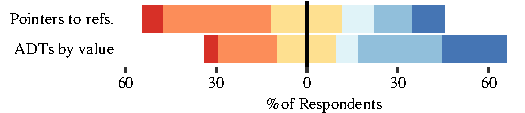
\includegraphics[width=\columnwidth]{figures/compiled/rq4_frequency_unsure.pdf}
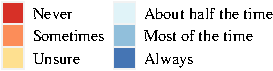
\includegraphics{figures/compiled/legends/legend_frequency_unsure_wrapped.pdf}
\end{figure}


The majority of interview participants and \ArrayItemRounded{*.feature.calling.foreign.functions}\% of survey respondents used Rust's foreign function interface (FFI). Multiple prior studies of Rust developers~\cite{holtervennhoff23,fulton21,astrauskas20} have also found that FFI use is common. Most participants found it difficult to reconcile the differences between Rust's memory model and foreign memory models. Participants reviewed the documentation and code from foreign libraries to ensure they were used safely, and they attempted to keep interoperation as straightforward as possible.

\FPeval{\createdbindings}{round(\ArrayItem{rq4.binding.method.i.generate.bindings.using.a.tool} + \ArrayItem{rq4.binding.method.i.write.bindings.manually} + \ArrayItem{rq4.binding.method.i.write.bindings.manually.and.generate.bindings.using.a.tool}
, 0)}

\subsubsection{Differing memory models}
Interview participants encountered several key differences between Rust and both C and C++ that made interoperation difficult. In C and C++, types can implement methods with varying thread-safety properties, but Rust's \code{Send} and \code{Sync} traits impose requirements on every behavior of a type. This made it difficult for one participant to encapsulate foreign types as wholly \code{Send} or \code{Sync} in Rust. They also noted that foreign libraries may have aliasing patterns that are fundamentally at odds with the borrow checker's restrictions. They observed that certain C APIs that receive source and destination pointers assume that the source and destination can alias, but aliasing and mutation are exclusive in Rust, so this pattern was difficult to encapsulate. Participants also noted that C allows unrestricted integer-to-pointer conversion, which is limited under Rust's strict provenance model, and that Rust's \code{Drop} semantics are different from a C++ destructor. 

To manage these differences, participants reviewed the documentation and implementation of foreign libraries to determine their safety requirements. The reverse of this situation occurred when participants exposed Rust libraries to languages with fewer safety guarantees. Implicit properties from Rust became documentation in other languages. 
\begin{pquote}{13}
...in Rust, you can trivially say, I'm going to return to you a thing, which just borrows my memory, and then you just can't access me while you're using that
...this is not very easily mappable into a C API, or rather you could do it, but then you have to read all this documentation...
\end{pquote}
Not all foreign APIs had were difficult to encapsulate, though. One participant observed that C APIs tend to expose pairs of initialization and cleanup functions for each type, which can be linked into the behavior of its Rust encapsulation. Others found that existing C APIs were easy to encapsulate since \ilquote{there [were] no complex lifetimes involved}{11}.

\subsubsection{Simple FFI} Participants attempted to keep interoperation with foreign code as straightforward as possible. When declaring bindings, one participant preferred  using primitive types and pointers over abstract data types like \code{Option} and \code{NonNull}, even though these types can be implicitly cast into raw pointers. They felt that these casts hid useful contextual information, so they preferred to use raw pointers explicitly.

\FPeval{\avoidedadts}{round(\ArrayItem{rq4.adts.avoided.always} + \ArrayItem{rq4.adts.avoided.most.of.the.time},0)}

A few participants indicated that they would avoid passing structs by value in certain situations. One of these participants found that certain Rust programs would behave incorrectly when structs were moved across a foreign boundary instead of copied, or if they had a destructor on the \CC{} side of the boundary. They typically avoided passing structs by value in either situation, and they recommended that \ilquote{...if you're doing FFI, the only things you should pass by value are \code{Copy} types}{2}. In most cases, participants felt comfortable passing structs by value if they were \code{Copy} and had equivalent layouts on each side of the boundary. However, as shown in Figure~\ref{fig:rq4:types}, nearly half (\avoidedadts\%) of survey respondents avoided passing abstract data types at least half of the time, if not more, suggesting that this practice is not universally followed.
 
In addition to limiting the use of certain types at boundaries, interview participants also attempted to minimize the interactions between each side of the FFI boundary. They thought that a \ilquote{very chatty API}{7} would be difficult to validate. One participant described the complexity of a foreign API in terms of the heap object graph that is exposed to Rust. They perceived that if the structure of the foreign heap is exposed in detail, then it will make safe encapsulations difficult to use.

\begin{pquote}{14}
It's hard to keep those objects around for very long unless you want all of your structs to end up with a bunch of lifetimes...
you don't want that...
it'll scare away new programmers for sure.
\end{pquote}
\FPeval{\avoidedrawasref}{round(\ArrayItem{rq4.raw.asref.avoided.most.of.the.time} + \ArrayItem{rq4.raw.asref.avoided.always},0)}
Survey respondents found it difficult to avoid converting foreign raw pointers into Rust's reference types; only \avoidedrawasref\% actively avoided this more than half of the time, as shown in Figure~\ref{fig:rq4:types}. This does not necessarily indicate that foreign heap objects tend to span FFI boundaries, but it does suggest that invalid pointer-to-reference casts may be a significant, unchecked source of undefined behavior, since Rust-specific development tools have limited support for foreign function calls. 

\rsqfour 
Developers perceived that certain API patterns were easy to encapsulate. However, unlike Holtervennhoff et al.~\cite{holtervennhoff23}, interview participants typically found it difficult to use foreign functions correctly because their aliasing and thread-safety properties were opaque and conflicted with the restrictions of the borrow checker and other Rust idioms. Participants minimized their interaction with foreign code to mitigate these differences. Some interview participants and survey respondents avoided passing structs by value, but survey respondents were not likely to avoid converting foreign raw pointers into safe references. 

\subsection{Validation}
\begin{figure}
\centering
\caption{How often survey respondents wrote tests for \unsafe code (``Write tests''), how often they audited their dependencies' use of \unsafe code(``Audit dependencies''), and how often participants executed their test cases in Miri if they had used the Miri at least once (``Run in Miri'').}
\label{rq5:tests-and-auditing}
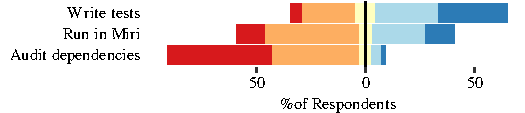
\includegraphics[width=\columnwidth]{figures/compiled/rq5_frequency.pdf}
\vskip 0.5em
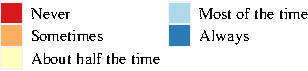
\includegraphics{figures/compiled/legends/legend_frequency_wrapped.pdf}
\end{figure}

Participants used a wide variety of development tools to assist with validating their design choices.

\FPeval{\tested}{round(\ArrayItem{rq5.tests.most.of.the.time} + \ArrayItem{rq5.tests.always}, 0)}
\FPeval{\miritested}{round(\ArrayItem{rq5.miri.test.sometimes} + \ArrayItem{rq5.miri.test.never}, 0)}

\paragraph{Dynamic Analysis} Most participants used dynamic bug-finding tools. Interview participants often mentioned Miri, AddressSanitizer, and Valgrind. Survey respondents most frequently used Miri (\ArrayItemRounded{rq5.tool.miri}\%), Valgrind (\ArrayItemRounded{rq5.tool.valgrind}\%), cargo-fuzz (\ArrayItemRounded{rq5.tool.cargo.fuzz}\%), and AddressSanitizer (\ArrayItemRounded{rq5.tool.addresssanitizer.(asan)}\%). Each remaining tool was used by less than 15\% of survey respondents. Three interview participants and \ArrayItemRounded{rq5.fuzzed}\% of survey respondents used fuzzing tools. One interview participant leveraged industry sponsorship to fuzz a JIT compiler for hours-on-end. Another participant implemented a B-Tree with optimizations for high-performance computing, and they used libFuzzer to perform differential testing~\cite{mckeeman98} against the BTree from Rust's standard library.

A majority (\tested\%) of survey respondents wrote tests for their \unsafe applications at least most of the time. However, Figure~\ref{rq5:tests-and-auditing} shows \miritested\% of participants who had used Miri only sometimes used it to validate their test cases, if at all. This may be due to Miri's lack of support for foreign functions, which was noted by the majority of interview participants. This was also a significant obstacle for survey respondents; \ArrayItemRounded{rq5.miri.deter.lack.of.support.for.foreign.function.calls}\% were deterred from using Miri because it could not call foreign functions. Respondents also avoided using Miri due to its performance (\ArrayItemRounded{rq5.miri.deter.slow.performance}\%) and lack of support for inline assembly (\ArrayItemRounded{rq5.miri.deter.lack.of.support.for.inline.assembly}\%). 
One participant had frequently encountered aliasing violations due to foreign function calls. They circumvented Miri's lack of FFI support by creating mocks of foreign functions, but this solution did not scale to programs with \ilquote{50,000 lines of code}{4} This participant and a few others were aware of the Krabcake project~\cite{krabcake}. Each was already using Valgrind with Rust codebases, and they perceived that Krabcake would be an ideal solution for overcoming each of Miri's limitations.


\FPeval{\debuggedyearly}{round(\ArrayItem{rq5.debugging.yearly} + \ArrayItem{rq5.debugging.less.than.once.a.year} + \ArrayItem{rq5.debugging.never}, 0)}
\FPeval{\debuggedmonthly}{round(\ArrayItem{rq5.debugging.monthly}, 0)}
\FPeval{\debuggeddaily}{round(\ArrayItem{rq5.debugging.daily}, 0)}

\paragraph{Debugging} Few interview participants reported using a debugger with Rust code. Only \debuggeddaily\% of survey respondents used a debugger daily, \debuggedmonthly\% used one monthly, and \debuggedyearly\% used one yearly at most, if at all. One interview participant had used both MSVC's debugger and LLDB, and while both worked, neither matched the quality of the other parts of the Rust toolchain, \ilquote{where you get all the bells and whistles that you want, and things just work nicely together}{3}. Mozilla's RR debugger~\cite{rr_debugger} was useful for one participant to resolve bugs found from fuzzing, but it was generally more common for participants to report using \ilquote{\code{printf}-style}{7} debugging.

\paragraph{Formal Methods} Few interview participants and only \ArrayItemRounded{rq5.formal}\% of survey respondents used tools that apply formal methods for static and dynamic verification. Interview participants mentioned using Kani, Prusti, and Crucible. Kani was useful for one participant, who needed to prove that a particular routine would never execute more than twice for any input. Another participant who had \ilquote{tried a bunch of the tools}{11} in this category found that Prusti was the most complete, but they felt that it would be more effective if these tools were \ilquote{inherently part of Rust}{11} so that they could \ilquote{hoist a lot of currently unsafe code into safe code}{11}. Of the survey respondents who had used formal methods tools, \ArrayItemRounded{rq5.formal.kani}\% had used Kani. Both Prusti and Creusot were used by \ArrayItemRounded{rq5.formal.prusti}\%, and Flux was used by \ArrayItemRounded{rq5.formal.flux}\%.

\FPeval{\noauditing}{round(\ArrayItem{rq5.auditing.frequency.never} + \ArrayItem{rq5.auditing.frequency.sometimes}, 0)}
\FPeval{\auditingtoolpercent}{round(\ArrayItem{rq5.auditing.tools.count} / \ArrayItem{responses.survey.valid} * 100, 0)}
\subsubsection{Auditing} Only a few interview participants described auditing \unsafe code. One participant would typically only examine their dependencies if they were curious about how they functioned. However, they did actively avoid dependencies that used outdated versions of Rust or deprecated features. Another participant was in the process of having a third-party institution examine their codebase to determine if they could reduce the amount of \unsafe code. Survey respondents also rarely audited their dependencies' use of \unsafe code; \noauditing\% audited their dependencies' use of \unsafe less than half the time, as shown in Figure~\ref{rq5:tests-and-auditing}. Additionally, only \auditingtoolpercent\% of respondents had used automated auditing tools. Of this subset, \ArrayItemRounded{rq5.auditing.tools.cargo-audit}\% had used cargo-audit, \ArrayItemRounded{rq5.auditing.tools.cargo-update}\% had used cargo-update, \ArrayItemRounded{rq5.auditing.tools.cargo-deny}\% had used cargo-deny, \ArrayItemRounded{rq5.auditing.tools.cargo-geiger}\% had used cargo-geiger, and only \ArrayItemRounded{rq5.auditing.tools.cargo-vet}\% had used cargo-vet.

\rsqfive Miri, Valgrind, cargo-fuzz, and AddressSanitizer were the most popular dynamic bug-finding tools that developers used with Rust applications. Though Miri was the most commonly used dynamic bug-finding tool, its performance and lack of support for key features deterred developers from using it. Holtervennhoff et al.~\cite{holtervennhoff23} found that developers rarely audit their code; our results illustrate that this is generally true. Developers rarely audited their dependencies' use of \unsafe code, and less than half had used auditing tools. 



\subsection{Community \& Culture}
Safety is one of the Rust community's core values. This informs positive practices, like safe encapsulation of \unsafe APIs, but can also be taken to extremes, as newcomers report unexpectedly harsh feedback from more experienced developers when they ask for advice on community forums. However, community resources are essential to understand the nuances of Rust's evolving semantics.
\subsubsection{A Preference for Safety}
Participants perceived that the Rust community has a strong preference for safety that affects tool design and development practices. Participants avoided exposing \unsafe APIs in libraries partly because of the perception that other Rust developers would otherwise avoid using their crate: \ilquote{everyone wants a safe interface... no one really wants to go use the \unsafe heavy ones}{9}.\FPeval{\avoidedunsafeapi}{round(\ArrayItem{rq3.avoided.most.of.the.time} + \ArrayItem{rq3.avoided.always}, 0)}
An overwhelming majority of survey respondents also preferred safe APIs; \avoidedunsafeapi\% would choose a safe API over an \unsafe alternative most of the time, if not always. One library author viewed safe encapsulation as an inevitable requirement. Even though exposing an \unsafe trait places the burden of responsibility on users, they would still blame the library.

\begin{pquote}{7}
So in theory, the burden of proof is on them, but also if they implement something improperly, then they're going to create a ticket because they'll be like, oh, ``I use your library and it's a fault.''
\end{pquote}

\subsubsection{A Stigma Against Unsafe}
Three participants observed a negative sentiment from other members of the Rust community toward any risk of undefined behavior. This was typically described in extreme terms: \ilquote{you have even the slightest concession to undefined behavior, and you've committed a crime against humanity}{7}. One participant perceived that this type of \ilquote{knee-jerk}{7} reaction was common toward newcomers asking for advice on community forums. They believed that these individuals were likely unaware of safer alternatives or the risks of their design choices. Fitting this pattern, another participant posted on a forum asking for advice on a potentially unsound optimization, and they received feedback that they felt was unnecessarily harsh.



\FPeval{\negativeview}{round(\ArrayItem{rq6.perception.general.extremely.negatively} + \ArrayItem{rq6.perception.general.somewhat.negatively}, 0)}

Survey respondents were prompted to evaluate their perception of the Rust community's view toward \unsafe code that they write, as well as \unsafe code in general. Most respondents were unsure about how \textit{their} \unsafe code was perceived, but \negativeview\% felt that the Rust community views \unsafe code at least somewhat negatively overall.

\subsubsection{Shifting Ground}
Interview participants had a collective sense of uncertainty about Rust's semantics. Participants perceived that Rust lacked a formal specification and that guidelines for \unsafe code were incomplete.

\begin{pquote}{10}
I think the biggest issue with Rust's {\normalfont \unsafe} isn't necessarily the tools, but just the spec\textemdash or, rather, the absence of the spec. If you write {\normalfont \unsafe} code today, you write it against the void.
\end{pquote}


\FPeval{\adequacymost}{round(\ArrayItem{rq6.adequate.most.of.the.time} +
\ArrayItem{rq6.adequate.always},0)}
\FPeval{\adequacyalways}{round(\ArrayItem{rq6.adequate.always},0)}

A few interview participants encountered situations where the precise definition of undefined behavior was still unclear. One participant needed to create a mutable reference to uninitialized memory, but this is considered undefined behavior by Rust's current semantics~\cite{ucg_ref_ub}. A similar debate occurred involving what one participant referred to as the \ilquote{ref header problem}{10}, which is also documented in an issue in the Unsafe Code Guidelines repository~\cite{ucg_ref_header_problem}. They wished to be able to take a reference to the first field of a product type and use it to create valid references to adjacent fields using integer offsets. This was considered undefined behavior under \textit{Stacked Borrows}, but it is now valid under \textit{Tree Borrows} semantics. Additionally, multiple participants were uncertain about how to handle the case when a program panics during a \code{Drop}. In contrast, the majority (\adequacymost\%) of survey respondents found that the Rust community's documentation and guidance was adequate for them to know how to use \unsafe code correctly most of the time, if not always. This suggests that concerns about Rust's evolving semantics, while important, are a niche issue for most developers that engage with \unsafe code.




\rsqfive Interview participants perceived that Rust developers prefer safe APIs, which incentivized them to avoid exposing \unsafe endpoints. The Rust community perceives \unsafe code somewhat negatively, and when reaching out to community members for feedback, newcomers are met with harsh reactions to their use of \unsafe code or their lack of caution toward undefined behavior. Developers rely on community guidance to understand what comprises undefined behavior, which has shifted as Rust has matured. However, Rust's documentation is typically adequate for them to know how to use \unsafe correctly.


